%%%%%%%%%%%%%%%%%%%%%%%%%%%%%%%%%%%%%%%%%%%%%%%%%%%%%%%%%%
% string.tex
% Authors: Alberto Ribon, Vladimir Uzhinsky, Gunter Folger
%%%%%%%%%%%%%%%%%%%%%%%%%%%%%%%%%%%%%%%%%%%%%%%%%%%%%%%%%%
\paragraph{Quark-gluon string models}
Two models based on quark-parton concepts were implemented in \Gfour{}, the
Quark-Gluon String (QGS) model
% proposed by A. Capella and A.B. Kaidalov
\cite{hadbib:FTF1,hadbib:FTF2} and the Fritiof (FTF) model.
% by Andersson et al.
\cite{hadbib:FTF3,hadbib:FTF4}.
The QGS model is described in \cite{bib:G4}.  A short description of the FTF
model is presented here, but more details are available in the \Gfour{} 
Physics Reference Manual \cite{hadbib:FTF19}.

%of the FTF model will be presented which is
%in production PhysicsLists of \Gfour used by LHC experiments.

The FTF model is used in \Gfour{} to simulate the following interactions:
hadron-nucleus at incident laboratory hadron momenta $>$ 3--5 GeV/c, 
nucleus-nucleus at incident laboratory hadron momenta $>$ 2--3 GeV/c/nucleon,
antibaryon-nucleus at all energies, and antinucleus-nucleus.
Because the model does not include multi-jet production in hadron-nucleon 
interactions, the upper limit of its validity range is estimated to be 1~TeV/c 
per hadron.

The modeling of hadron-nucleon interactions in the FTF model includes the
simulation of elastic scattering, binary reactions such as 
$NN\rightarrow N\Delta$ and $\pi N\rightarrow \pi \Delta$, single diffractive 
and non-diffractive events, and annihilation in anti-baryon-nucleon interactions.
Interactions proceed by the production of one or two unstable objects called 
quark-gluon strings.  If only one string is created, the process is called 
diffraction dissociation.  

In the \Gfour{} implementation single diffraction dissociation is simulated 
separately from non-diffractive interactions.  A special function which 
corresponds to a weighted simulation of the diffraction dissociation was
introduced to perform this separation.  In most other Fritiof-based models 
this separation is governed by a single parameter, which is not sufficient for
a correct description of the large set of experimental data. 

Once formed, strings may interact with other nucleons in hadron-nucleus and 
nucleus-nucleus collisions, producing additional strings.  Strings with 
sufficiently large mass ($>$ 1.2~GeV) may in general have kinks, which are
treated as emitted gluons which decay into quark-antiquark pairs.  This feature
is required in order to reproduce particle multiplicities observed in hadronic 
interactions at high energies.  However, the current FTF implmentation does not 
handle kinks, hence the TeV/c upper limit.  

% Because multi-gluon production in elementary interactions is
% not included in FTF, the upper limit of the model's validity is estimated to be 
% 1~TeV, sufficient for most applications of \Gfour{}.

Hadron-nucleon scattering within the model uses the elastic and inelastic cross 
sections taken from the CHIPS parameterizations \cite{hadbib:CHIPS}. 
Cross sections for binary reactions and diffraction dissociation were implemented
directly in the FTF model as parameterizations of data.  Here the cross sections
for the unstable objects were taken to be the same as those for stable objects
with the same quark content.  

Once the unstable objects are produced, the LUND string fragmentation model is 
used to decay them \cite{hadbib:FTF7}.  The parameters of this model were tuned
to experimental data and the available phase space was restricted to take into 
account low mass string fragmentation.  The formation time of hadrons was also 
applied.

To simulate hadron-nucleus and nucleus-nucleus scattering it is necessary to 
embed the hadron-nucleon interaction in the nuclear environment.  This was done
by first assuming a Woods-Saxon parameterization of the one-particle nuclear 
density for medium and heavy nuclei and a harmonic oscillator shape for light 
nuclei.  Center-of-mass correlations and short-range nucleon-nucleon 
correlations were taken into account.  A simplified Glauber model was used to 
sample the multiplicity of intra-nuclear collisions.  Screening was not 
considered; estimates and data indicate that it decreases the total 
hadron-nucleus cross sections by 3--5\%, while the inelastic hadron-nucleus 
cross sections are practically unchanged \cite{hadbib:Alvi}.  Hence any effect 
on the multiplicity of produced particles is expected to be small.

The number of string objects in non-diffractive interactions is proportional to
the number of participating nucleons. Thus, multiplicities in hadron-nucleus and
nucleus-nucleus interactions are larger than those in elementary interactions.
It is assumed that the reaction creating unstable strings in hadron-nucleus
collisions is analogous to that in nucleus-nucleus collisions.

It is known that the Glauber approximation used in this and other string models
does not provide enough intra-nuclear collisions for a correct description of
nuclear destruction.  Traditional cascade models would fulfill this need, except 
that they produce too many particles.  Reggeon theory has been proposed to solve
this problem \cite{hadbib:FTF18}, but the detailed calculation required was not
appropriate for a reasonably fast computer code.  A simplified implementation in
\Gfour{} assumes \cite{hadbib:FTF10} that participating nucleons predicted by the 
Glauber approximation initiate low energy reggeon exchanges in the spectator 
part of a target nucleus.  This reggeon theory inspired model (RTIM) provides 
the right number of fast nucleons ejected during nuclear destruction and 
describes secondary particle intra-nuclear cascading \cite{hadbib:FTF8}.   

The collective nature of nuclear destruction led to the introduction of a new
"Fermi motion" \cite{hadbib:FTF9,hadbib:FTF10} simulation which is a refined 
algorithm for putting involved nucleons on the mass-shell.  As shown in 
Figure~\ref{had:FTFfig1}, this provides sufficient agreement with experimental
data in the transition region, around 3~GeV/c.

When the cascading is finished, the excitation energies of residual nuclei are
estimated in the ``wounded nucleon'' approximation \cite{hadbib:FTF11}. This 
allows for a direct coupling of the FTF model to the \Gfour{} precompound model
and its nuclear fragmentation sub-models.  The determination of the particle
formation time also allows coupling of the FTF model to the \Gfour{} Binary 
cascade model \cite{hadbib:FTF12}.

%The Ultra-Relativistic Quantum Molecular Dynamic model (UrQMD) \cite{hadbib:FTF13}
%simulates the binary reactions, but it seems to as that their cross sections are
%not tuned quite well. 

% An effort is underway to fit the cross sections in the FTF model, but up to
% now only low mass resonances have been considered. It is thus expected that the
% FTF model is not entirely correct at projectile energies below 3--5 GeV.

% A peculiarity of the \Gfour Fritiof model implementation is the separate 
% simulation of the single diffraction dissociation and non-diffractive 
% interactions. In most Fritiof-based models the separation between the processes
% is governed by a single parameter.  This, however, is not sufficient for a 
% correct description of the large set of experimental data.  A special function
% for this separation was therefore introduced, which corresponds to a weighted 
% simulation of the diffraction dissociation.

Two additional innovations were made in the FTF model, one dealing with low-mass
strings and the other making multiplicity corrections in hadron-nucleus and
nucleus-nucleus reactions.
   
All Monte Carlo event generators are challenged with the correct treatment 
of low mass strings. Such a string is typically handled by first checking that
it can decay into two low mass particles. If it can, the decay is simulated;
otherwise, the string is converted into a hadron.  This step violates 
energy-momentum conservation and the momenta of all other produced particles
must be adjusted to correct for this.  In the FTF model all strings with 
sufficiently large mass are allowed to decay to two particles.  As a result, the
cross sections of the reactions $\bar p+p \rightarrow \bar n+n$, 
$\bar p+p \rightarrow \bar \Lambda+\Lambda$, and so on, are reproduced. In the 
case of a two-particle decay, all possible final states are considered, and one 
is chosen according to its phase space volume. For other final states, standard 
string fragmentation or direct production of a hadron is possible.  

% Strings with sufficiently large mass ($>$ 1.2 GeV) can have a kink. The kink is
% treated as a gluon which decays into a quark-antiquark pair. This is needed
% to reproduce particle multiplicities observed in hadronic interactions. The 
% UrQMD model \cite{hadbib:FTF13}, for example, does not consider kinky strings,
% while the Hijing model \cite{hadbib:FTF14} assumes copious gluon production in 
% hard and semi-hard interactions. The Fritiof 7.0 model \cite{hadbib:FTF15} also
% considers gluon production. Because multi-gluon production in elementary 
% interactions is not included in the \Gfour FTF model, its upper limit of 
% application is estimated to be 1 TeV, sufficient for most applications of \Gfour.

Multiplicity corrections in hadron-nucleus and nucleus-nucleus interactions are 
necessary when computing the number $N_{bin}$ of intra-nuclear collisions.  The
distribution of $N_{bin}$ is usually obtained by applying the asymptotic AGK 
cutting rules \cite{hadbib:FTF16} to the Glauber amplitude for elastic 
scattering.  These rules must be corrected for finite energies. Because there is
no defined prescription for making these corrections, a phenomenological 
approach, taking into account formation time and using HARP-CDP data 
\cite{hadbib:FTF17}, was adopted.

%{\bf suggest to remove all this and quote an article with details:\\
%As known, a simple cascade model considers only pions and nucleons. Due to this
%it cannot work when resonance production is a dominating process in hadronic
%interactions. But if the energy is sufficiently low the resonances can decay
%before a next possible collision, and the model can be valid.
%  OK above ??
% Let $p$ be the momentum
%of a produced resonance ($\Delta$). The average life time of the resonance in
%its rest frame is $1/\Gamma$. In the laboratory frame the time is
%$E_\Delta/\Gamma m_\Delta$. During this time, the resonance will fly a distance
%$\bar{l}=v\ E_\Delta/\Gamma m_\Delta=p/\Gamma m_\Delta$. If the distance is less
%than an average distance between nucleons in nuclei ($\bar{d}\sim 2$ fm),
%the model can be applied. From the condition, we have:
%$
%p\leq \bar{d}\ \Gamma m_\Delta \sim 1.5
%$
%(GeV/c).
%
%Direct $\Delta$-resonance production takes place in $\pi N$ interactions at low energies.
%Thus the model cannot work well at a momentum of pions above 2 GeV/c. In nucleon-nucleon
%interactions, due to momentum transfer to a target nucleon, the boundary can be higher.
%
%Returning back to the FTF model, let us assume that projectile originated strings
%have an average life time $1/\Gamma$, and an average mass $m^*$. The strings can
%interact on average with $\bar{l}/\bar{d}=p/\Gamma m^*\bar{d}=p/p_0$ nucleons.
%Here $p_0$ is a new parameter. According to our estimates it is about 2 -- 3 GeV/c.
%Thus, we can assume that at any energy there is a maximum number of intra-nuclear
%collisions in the FTF model -- $\nu_{max}=p/p_0$.
%This restriction is implemented in the current version of the FTF model, and puts
%a low boundary of the model application region to 3--5 GeV/c. For the determination
%of the $p_0$ parameter we used the HARP-CDP data \cite{hadbib:FTF17}.
%
%As known, the Glauber approximation used in the Fritiof model and in the other
%string models does not provide enough intra-nuclear collisions for a correct
%description of a nuclear destruction. Additional cascading in nuclei is needed!
%Usage of a standard cascade for secondary particle interactions leads to a large
%multiplicity of produced particles. Usually, it is assumed that an inclusion of
%a secondary particle's formation time can help to solve this problem, but there
%is no unified solution. The concept of the formation time was criticized in
%the paper \cite{hadbib:FTF18} where the intra-nuclear cascade was considered
%from the reggeon theory point of view. Because we were not be able to implement
%a complicated reggeon calculation scheme, we have assumed \cite{hadbib:FTF10}
%that participating nucleons predicted by the Glauber approximation initiate
%low energy reggeon exchanges in a spectator part of a target nucleus (reggeon
%cascading). This provide us with an enough amount of fast nucleons ejected at
%a target nucleus destruction.
%
% This collective nature of the destruction
%pushed us to introduce a new "Fermi motion" simulation which is a refined
%algorithm of putting of involved nucleons onto mass-shell.  All of these
%allowed us to obtain a smooth transition from the FTF model and low energy
%Bertini and Binary cascade models of \Gfour (see Fig.~\ref{had:FTFfig1}a).
%
%The main problem now is an accounting of the diffraction dissociation in
%hadron-nucleus and nucleus-nucleus interactions. A transition of a projectile
%particles into a diffractive system and back during elastic scattering on a nucleus
%has to be suppressed by the nuclear form-factor. Due to this a projectile
%diffraction dissociation in inelastic interactions has to be also suppressed
%according to the reggeon phenomenology. One cannot apply this consideration
%to a target nucleon diffraction, and one can assume that they can dissociate.
%But the calculations presented in Fig.~\ref{had:FTFfig1} were done without
%the suppression for $p{\rm Ta}$ interactions, and with full suppression for
%$\pi {\rm Ta}$ interactions. Another choice makes the description worse.
%The question is now under the study.
%}

\begin{figure}
\centering
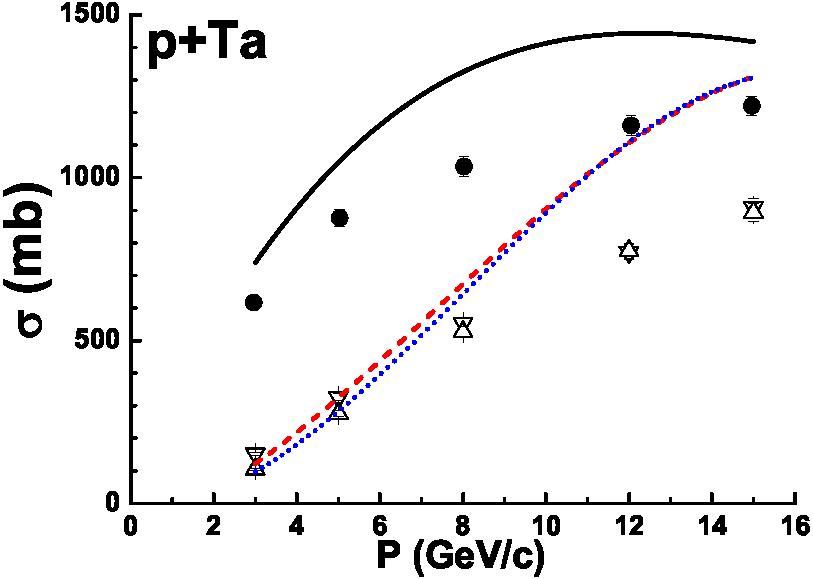
\includegraphics[height=1.8in,width=1.70in]{figures/FTFfig1_1.pdf}
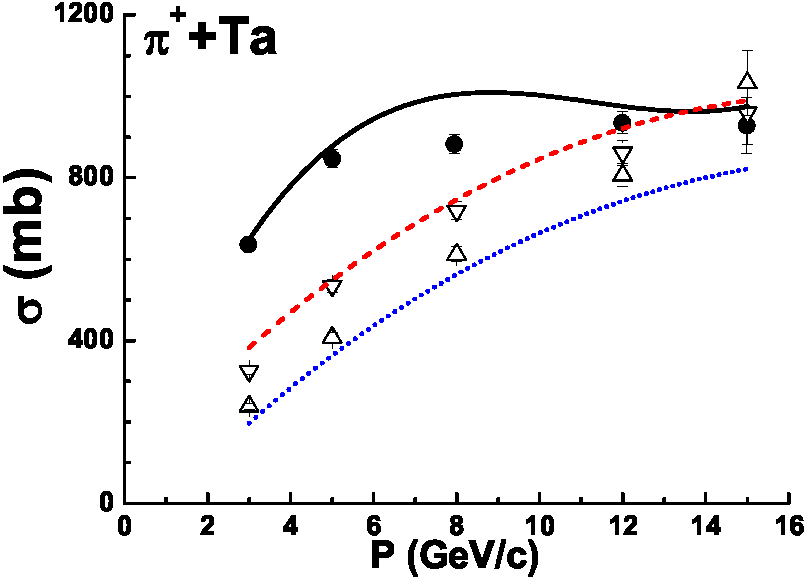
\includegraphics[height=1.8in,width=1.7in]{figures/FTFfig1_2.pdf}
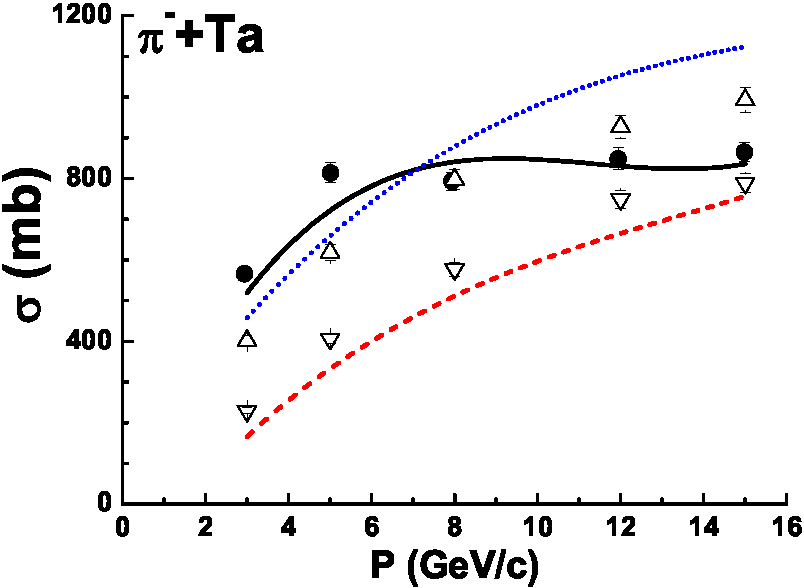
\includegraphics[height=1.8in,width=1.7in]{figures/FTFfig1_3.pdf}
\caption{Inclusive cross sections for $p$, $\pi^+$ and $\pi^-$ production in
         $p{\rm Ta}$, $\pi^+{\rm Ta}$ and $\pi^-{\rm Ta}$ interactions as a 
         function of projectile hadron momentum.  Data from the HARP-CDP 
         group \protect{\cite{hadbib:FTF17}} are shown as closed circles for
         protons and up- and down-triangles for $\pi^+$ and $\pi^-$,
         respectively.  Lines are FTF model calculations: solid for protons,
         dashed and short-dashed for $\pi^+$ and $\pi^-$, respectively.}
\label{had:FTFfig1}
\end{figure}


